% Generated by scripts/txt2tex.py from chapters/appendix.txt. Edit the TXT, not this file.
\chapterlayout{appendix}
\chapterquestion{אם מכונות כתבו את הספר הזה, מי בדק את המכונות?}
\chapter{כך נוצר הספר שאתם קוראים}\label{ch:appendix}
\section{צוות שאינו נפגש לעולם}
לאורך שבעה פרקים ליווינו את הקוראת מהשאלה על הבצק ועד ההחלטה מה לעשות בתשובה. הספר עצמו עבר מסע דומה, ומעל כל המערכות עמד אדם.
בשלב כתיבת הפרקים ביצעו את העבודה ארבעה סוכנים, כלומר ארבעה מופעים של מערכת בינה מלאכותית אחת (Claude Code), שלכל אחד מהם הוגדרו תפקיד, כלים מותרים וקבצים שמותר לו לכתוב \projref{\nolinkurl{agents/orchestrator_agent.md}}. סוכן המחקר (Research) חיפש מקורות ואימת אותם. סוכן הכתיבה (Writer) ניסח את הפרקים בלי שום גישה לרשת, כדי שלא יוכל "למצוא" מקור שאינו קיים. סוכן הביקורת (Reviewer) בדק, נתן ציון ופסק אם הפרק צריך תיקון, אבל לא הורשה לערוך את הטקסט בעצמו \projref{\nolinkurl{docs/PROMPT_HISTORY.md}, רשומה 002}. מעל שלושתם פעל סוכן-העל (Orchestrator): תכנן, הפעיל, העביר ובדק. בשלב ההפקה הצטרף אליהם סוכן חמישי, ועל כך בהמשך.
דמיינו מערכת עיתון שבה הכתב, בודק העובדות והעורך יושבים בחדרים נפרדים ואינם מכירים זה את זה. כל דף עובר דרך שולחן אחד במרכז, ושם מחליטים לאן הוא ממשיך. זה המבנה שנקרא כוכב (hub-and-spoke): תת-סוכן אינו פונה לתת-סוכן אחר, וכל מסירה עוברת דרך סוכן-העל \projref{\nolinkurl{agents/orchestrator_agent.md}}. ה"דף" הוא קובץ: רשימת מקורות, פרק או דוח ביקורת. כל סוכן מתחיל בהקשר נקי וקורא רק את מה שהועבר אליו.
הסדר קבוע: מחקר, אחריו כתיבה, ואחריה ביקורת. פרק בלי מקורות מאומתים לא נשלח לכתיבה \projref{\nolinkurl{agents/orchestrator_agent.md}}. בשלב המחקר הופעל סוכן המחקר על שבעת הפרקים במקביל, ואחר כך בהרצת איחוד שבנתה אינדקס של 73 רשומות, ש-61 מהן שמישות לכתיבה \projref{\nolinkurl{docs/PROMPT_HISTORY.md}, רשומה 005; agents/runs/research\_all\_r1.md}.
\begin{figure}[htbp]
\centering
% Figure A.1 (נ.1): four agents and one table in the middle (star architecture, agents/orchestrator_agent.md).
\begin{bookdiagram}[x=1cm,y=1cm]
  \tikzset{ag/.style={blk,draw=turquoise,line width=1.1pt,text width=2.7cm,minimum height=11mm},
           lbl/.style={font=\scriptsize,fill=white,inner sep=1pt}}
  \node[blk,draw=midnight,line width=1.6pt,text width=3.3cm,minimum height=13mm,font=\headingfont] (o) at (0,0) {סוכן-העל\\(Orchestrator)};
  \node[ag,draw=midnight] (u) at (0,3.0) {המשתמשת};
  \node[ag] (r)  at (5.4,-3.2) {Research};
  \node[ag] (w)  at (0,-3.6)   {Writer};
  \node[ag] (v)  at (-5.4,-3.2) {Reviewer};
  \draw[{Stealth[length=2.4mm]}-{Stealth[length=2.4mm]},line width=1pt,midnight] (u) -- node[lbl,right=2mm] {החלטות ואישורים} (o);
  \draw[flow] (o) -- node[lbl,sloped] {משימה $\leftarrow$ מקורות} (r);
  \draw[flow] (o) -- node[lbl] {משימה $\leftarrow$ פרק} (w);
  \draw[flow] (o) -- node[lbl,sloped] {משימה $\leftarrow$ דוח ו-VERDICT} (v);
  % revision loop (dashed, violet)
  \draw[loop] (v.north) to[out=95,in=180] node[pos=0.5,above left,text=violet,font=\scriptsize\headingfont] {REVISE} (o.west);
  \draw[loop] (o.south east) to[out=-20,in=150] node[pos=0.55,above right,text=violet,font=\scriptsize] {תיקון לפי קטגוריית הליקוי} (r.north west);
  \node[text=violet,font=\footnotesize\headingfont] at (-5.4,-4.45) {עד 3 סבבים};
  % PASS exit
  \node[blk,draw=midnight,text width=2.6cm] (p) at (6.0,0.6) {PASS: היחידה עוברת};
  \draw[-{Stealth[length=2.6mm]},line width=1.2pt,midnight] (o.east) -- (p.west);
  \fill[gold] ($(p.west)+(-0.25,0)$) circle (2pt);
  % documentation store
  \node[cylinder,shape border rotate=90,draw=midnight,fill=midnight!6,aspect=0.25,minimum width=2.9cm,minimum height=1.4cm,align=center,font=\scriptsize]
     (db) at (-5.6,1.2) {\texttt{agents/runs/}\\ו-\texttt{PROMPT\_HISTORY}};
  \draw[-{Stealth[length=2.4mm]},line width=0.8pt,midnight,dashed] (o.north west) -- node[lbl,above,sloped] {תיעוד} (db.east);
\end{bookdiagram}

\caption{ארבעה סוכנים ושולחן אחד במרכז}\label{fig:A.1}
\figurenote{מקור: agents/orchestrator\_agent.md}
\end{figure}
\section{שער שאינו סומך על אף אחד}
אחרי כל הרצה עצר סוכן-העל ובדק את התוצר. שלוש בדיקות חזרו שוב ושוב. הראשונה: האם הסוכן נגע רק בקבצים שלו. את זה בדקה הפקודה git status, ולפני שהקבצים נכנסו למעקב, השוואה של טביעות אצבע דיגיטליות (MD5) לכל קובץ \projref{\nolinkurl{agents/runs/smoke_test/README.md}}. השנייה: ספירת מילים בקוד Python. כבר בניסוי הראשון התברר שכלי הספירה הרגיל טועה בעברית, וספר 22 מילים במקום 117 \projref{\nolinkurl{agents/runs/smoke_test/README.md}}. גם סוכן הכתיבה אינו סופר במדויק: על פרק 1 הוא דיווח 1,170 מילים, והשער מצא 1,247 \projref{\nolinkurl{docs/PROMPT_HISTORY.md}, רשומה 007}. השלישית: כל מזהה מקור בפרק הושווה לאינדקס, כדי שלא יופיע ציטוט שאין מאחוריו רשומה \projref{\nolinkurl{agents/runs/writer_ch03_r2.md}}.
השער תפס גם חורים בתוכן. בסבב המחקר הראשון לפרק 7 התברר שאין בין המקורות אף מחקר אמפירי על השפעת הכלים על לימודים. סבב נוסף הוסיף 4 רשומות, ובהן שני מחקרים שעברו ביקורת עמיתים \projref{\nolinkurl{docs/PROMPT_HISTORY.md}, רשומה 005}.
\section{לתקן, לבדוק שוב, ולדעת מתי לעצור}
כל דוח ביקורת מסתיים בשורה אחת שמכונה יכולה לפענח: VERDICT: PASS או VERDICT: REVISE. די בליקוי אחד בחומרה קריטית או בינונית כדי שהפסק יהיה REVISE. את ההחלטה לאן הפרק חוזר מקבל סוכן-העל: את הליקויים בקטגוריית "מקורות" הוא מנתב לסוכן המחקר, ואת כל השאר לסוכן הכתיבה. ואם אחרי 3 סבבים אין עדיין PASS, ההחלטה עוברת לאדם \projref{\nolinkurl{agents/orchestrator_agent.md}}.
\begin{behindbox}{הסבב הראשון שהושלם}
לפני שנכתבה מילה בספר נערך ניסוי הרצה קטן (smoke test). סוכן המחקר מצא מאמר על רשתות נוירונים, סוכן הכתיבה ניסח פסקה של 117 מילים, וסוכן הביקורת נתן לה 80 מתוך 100 ופסק REVISE: המונח "התפשטות לאחור" לא הוסבר \projref{\nolinkurl{agents/runs/smoke_test/README.md}}. הליקוי סווג כבעיית סגנון, אבל ההסבר החסר דרש עובדה חדשה, ולכותב אין רשת, ולכן הפסקה עברה קודם לסוכן המחקר. בסבב השני היו בה 162 מילים, והיא קיבלה 92 ו-PASS \projref{\nolinkurl{agents/runs/smoke_test/README.md}}.
\end{behindbox}
אותו דפוס חזר בספר עצמו. כל שבעת הפרקים הוחזרו לתיקון בסבב הראשון, וכולם עברו בהמשך. פרק 5 עלה מ-81 ל-95, פרק 7 מ-90 ל-99, ופרקים 3 ו-4 מ-88 ל-97 \projref{\nolinkurl{agents/runs/m3_summary.md}}. פרק 1 עבר שלושה סבבים, 84, 92 ו-98 \projref{\nolinkurl{agents/runs/m3_summary.md}}. בסבב הראשון שלו מצא המבקר שלושה משפטים שהיו כמעט תרגום מילולי של תקציר מאמר: עם ייחוס, אבל בלי סימון ציטוט. הוא סיווג זאת ליקוי מקוריות בחומרה בינונית \projref{\nolinkurl{agents/runs/review_ch01_r1.md}}, ובסבב הבא נכתבה הפסקה מחדש \projref{\nolinkurl{agents/runs/review_ch01_r2.md}}.
\section{המספר שהמאמר עצמו טעה בו}
הסיפור המלמד ביותר התרחש בפרק 2, על מערכות מסחריות לסיווג פנים. בסבב השני של הפרק הוסיף סוכן הכתיבה לאחת התיבות השוואה בין מאגרי תמונות, ובה הנתון שבמאגר Adience נשים כהות עור הן 4.4\% בלבד \projref{\nolinkurl{agents/runs/review_ch02_r2.md}}. המספר הגיע מרשומת המקור, והרשומה לקחה אותו מכיתוב של איור במאמר. סוכן הביקורת לא הסתפק בכיתוב. הוא חילץ את הטקסט מקובץ המאמר, קרא את העמודות שבאיור עצמו ואת גוף הסעיף, ומצא ששם 4.4\% שייך למאגר אחר, IJB-A, ואילו ב-Adience השיעור הוא 7.4\% \projref{\nolinkurl{agents/runs/review_ch02_r2.md}}. המאמר סתר את עצמו, והכיתוב הוא שטעה. הפרק קיבל 94 ונשלח שוב לתיקון \projref{\nolinkurl{agents/runs/m3_summary.md}}.
כאן הלולאה התפצלה. הניסוח חזר לכותב, והרשומה, שעלולה הייתה להטעות גם פרקים אחרים, נשלחה לסוכן המחקר. ההנחיה אליו הייתה חדה: לא לסמוך על המספרים של המבקר, אלא לחזור למאמר הרשמי ולבדוק בעצמו \projref{\nolinkurl{agents/runs/research_ch02_r2.md}}. הוא מצא אותה סתירה, תיקן את הרשומה ותיעד את הטעות שבכיתוב. בסבב השלישי עבר הפרק בציון 98 \projref{\nolinkurl{agents/runs/review_ch02_r3.md}}. שלושה סוכנים, ואף אחד מהם לא נדרש להאמין לאחר על סמך המילה שלו.
\section{כשהחוט נקרע}
העבודה נקטעה באמצע יותר מפעם אחת. בניסוי ההרצה התנתק החיבור לשרת המודל אחרי שדוח הביקורת הראשון התקבל, ולפני שנכתב קובץ התיעוד שלו. סוכן-העל לא סמך על הזיכרון: הוא השווה את טביעות האצבע של הקבצים לתמונת המצב שנשמרה וקרא שוב את ה-VERDICT והציון. כל התוצרים היו שלמים וחסר רק קובץ אחד; הוא השלים אותו והמשיך, בלי להפעיל מחדש אף סוכן שכבר סיים \projref{\nolinkurl{agents/runs/smoke_test/README.md; docs/PROMPT_HISTORY.md}, רשומה 004}. הלקח נכתב אז לפרוטוקול: אחרי ניתוק מאבחנים לפי מה שיש בדיסק, ומשלימים רק את מה שחסר \projref{\nolinkurl{agents/orchestrator_agent.md}}.
אחר כך נעצר סוכן הכתיבה באמצע תיקון פרק 3 בגלל מגבלת שימוש (HTTP 429), ואחרי האיפוס סיים את כל 8 הליקויים \projref{\nolinkurl{agents/runs/writer_ch03_r2.md}}. בשלב התיקונים האחרון פקעה ההתחברות באמצע הרצה של סוכן המחקר. לפי git status לא נכתב אף קובץ, ואחרי התחברות מחדש חודש אותו סוכן מהנקודה שבה עצר \projref{\nolinkurl{docs/INCIDENTS.md}, IR-18; agents/runs/research\_m5b\_r1.md}. הכלל בכל המקרים זהה: בודקים מה קיים בפועל, לא חוזרים על עבודה שסומנה כגמורה, ומחדשים את אותו סוכן כשאפשר \projref{\nolinkurl{docs/STATUS.md}}. כל תקלה כזאת נרשמה ביומן אירועים, שמונה כיום 19 רשומות. כל רשומה מפרידה בין עובדות להשערות, ומסתיימת בצעד שימנע חזרה \projref{\nolinkurl{docs/INCIDENTS.md}}.
\begin{thinkbox}
בספר הזה מכונות בדקו מכונות, והמבקר הוא מופע של אותה מערכת שכתבה. האם זו ביקורת בלתי תלויה באמת? כמה מן העצמאות נובעת מהקשר נפרד, מכלים מוגבלים ומקבצים שכל אחד יכול לפתוח, וכמה ממנה היא רק אשליה של סדר? ואילו החלטות, לדעתכם, אסור למסור לאף לולאה?
\end{thinkbox}
\section{מהטקסט אל הדף}
בשלב ההפקה רץ ניסוי זיהוי הספרות של פרק 5, האיורים נוצרו בקוד, וסקריפט המיר את הפרקים ל-TeX. עד גרסה 1.4 של מסמך הדרישות תוכנן הספר להידור ב-XeLaTeX. בגרסה 1.5, לפי דרישות המרצה שהעבירה המשתמשת, הוא עבר ל-LuaLaTeX, עם biber, ציטוטים בסגנון IEEE ותבנית עיצוב משלו \projref{\nolinkurl{docs/PRD.md; latex/aibook.cls}}. למעבר היה מחיר, כי LuaLaTeX מטפל בכיווניות אחרת. תיבות, תרשימים ופסי כותרת זזו אל מחוץ לעמוד \projref{\nolinkurl{docs/INCIDENTS.md}, IR-05}, ובתוך טקסט עברי התהפכה הליגטורה fi, כך שהמילה artificial יצאה artfiicial \projref{\nolinkurl{docs/INCIDENTS.md}, IR-10}. הפתרון הוטמע בתבנית עצמה: מסגרת משמאל לימין, שבתוכה התוכן חוזר לימין לשמאל. מאז עברה התבנית שלוש גרסאות, עד 1.2.0.
באותו שלב התרחב הצוות. סוכן הביקורת קיבל תפקיד נוסף, מאתר ליקויים (Detector), שבודק את הספר המהודר ולא רק את הטקסט. לצידו נוסף סוכן חמישי, מתקן (Fixer), שמתקן במינימום שינוי לפי דוח המאתר \projref{\nolinkurl{agents/fixer_agent.md}}. ליקוי שיטתי, שחוזר מאותה סיבה בפרקים רבים, אינו מתוקן בטקסט. המתקן מסלים אותו לסוכן-העל, והוא מתוקן בכלי שיצר אותו: בתבנית, בממיר או בסקריפט. כך התיקון נעשה פעם אחת, ולא שבע.
גם שגרות העבודה נשמרו כקבצים: 13 מיומנויות (Skills), חמישה נהלים לסוכנים ושמונה בדיקות איכות, כמו כיווניות (qa-BiDi), טבלאות ועימוד [.claude/skills/]. הבדיקות הן קוד, ולא סוכנים נפרדים. פקודה אחת, qa-super, מריצה את כולן וכותבת דוח אחד, והמאתר מפעיל אותה [scripts/qa.py]. ובכל זאת הן תנאי הכרחי ולא מספיק: שלושה ליקויי תבנית חמקו מהן ונתפסו רק בעין \projref{\nolinkurl{docs/INCIDENTS.md}, IR-09 עד IR-11}, וכל ליקוי כזה הפך לבדיקה חדשה.
\section{עין מבחוץ}
איור~\ref{fig:A.2} מרכז את ציוני הפרויקט: לכל יחידה, הציון בסבב הביקורת הראשון מול הציון בסבב האחרון. חשוב לקרוא אותו נכון. אלה ציוני ביקורת פנימית שנתן סוכן הביקורת, ולא ציון של מרצה או של בודק אנושי \projref{\nolinkurl{python/data/review_scores.csv}}. בסבב הראשון נעו הציונים בין 80 ל-92, ובאחרון בין 92 ל-99. גם הספר המהודר עלה בבדיקת המאתר מ-84 ל-96.
\begin{figure}[htbp]
\centering
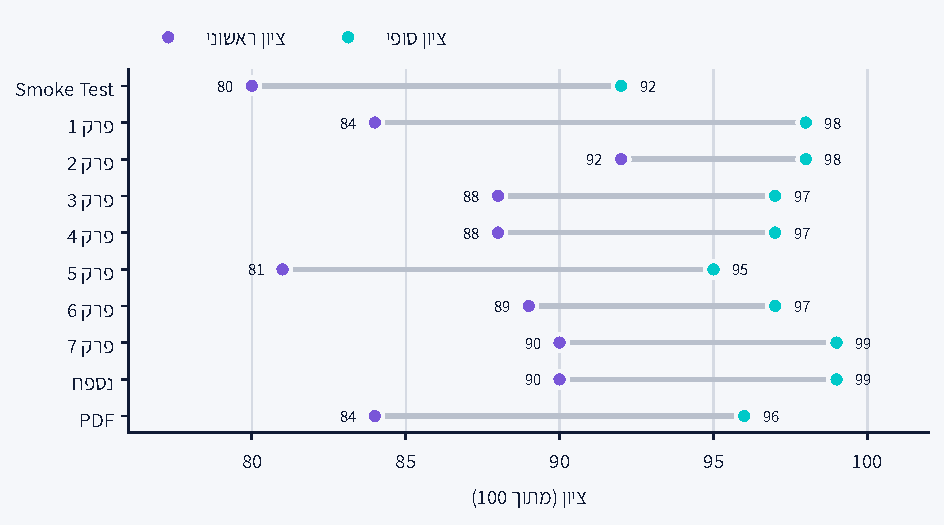
\includegraphics[width=\linewidth]{assets/charts/figA_2_scores.pdf}
\caption{ציוני הביקורת הפנימית של הסוכנים, סבב ראשון מול סבב אחרון}\label{fig:A.2}
\figurenote{מקור: python/data/review\_scores.csv}
\end{figure}
אבל ציון 96 ופסק PASS אינם סוף פסוק. אחרי שלב ההפקה העבירה המשתמשת את הספר, גרסה 0.9 בת 46 עמודים, לביקורת חיצונית ב-ChatGPT, מחוץ למערכת הסוכנים \projref{\nolinkurl{prompts/12_m5b_m6_external_review.txt}}. המבקר החדש מצא ליקויים שהלולאה הפנימית החמיצה. בעימוד: מספור עמודים, שטחים לבנים, תיבות סיכום בעמודים כמעט ריקים, חפיפות בתרשים 2.1, סימוני LaTeX גולמיים, עברית הפוכה בגרפים והביבליוגרפיה \projref{\nolinkurl{docs/INCIDENTS.md}, IR-14 עד IR-17}. ובמדע: מקור מדויק לפונקציית tanh וקביעות גורפות מדי עליה, ערבוב בין שגיאת הכללה לפער הכללה, הגדרות לא מדויקות של התאמת יתר ותת-התאמה, תיאור של קבוצת הבדיקה שלא תאם את הקוד במלואו, וההסתברויות של "כל השאר" בגרף הטמפרטורה.
גם להערות האלה לא האמינו על סמך המילה. סוכן המחקר חזר למקורות ומצא שבעניין שגיאת ההכללה הביקורת צודקת רק בחלקה: יש חוקרים שמכנים כך את הפער עצמו, אבל "פער הכללה" חד יותר, ובו בחר הספר \projref{\nolinkurl{agents/runs/research_m5b_r1.md}}. רוב ליקויי העימוד היו שיטתיים, ולכן תוקנו בכלים וקיבלו בדיקות חדשות. והלקח: מודל אחר, שלא השתתף בכתיבה, ראה מה שמערכת שבודקת את עצמה לא ראתה.
\section{האדם שמעל הלולאה}
המבנה עצמו נולד מדרישה של המשתמשת שהובילה את הפרויקט: ארבעה סוכנים ומבנה כוכב \projref{\nolinkurl{docs/PROMPT_HISTORY.md}, רשומה 002}. היא בחרה את הפלטה ואת רוח הכתיבה, והחליטה שהנספח הזה ייכתב \projref{\nolinkurl{docs/PROMPT_HISTORY.md}, רשומות 006–007}. פרק 1 נכתב לבדו, והעבודה נעצרה. רק אחרי שאישרה את הפרק ואת הסגנון נכתבו שאר הפרקים \projref{\nolinkurl{docs/PROMPT_HISTORY.md}, רשומות 007–008}.
הסוכנים אינם צוות של אנשים. הם מופעים של מערכת בינה מלאכותית, והראיה למה שעשו אינה ההצהרות שלהם אלא התיעוד. כל פרומפט וכל פלט גולמי נשמרו בתיקיית agents/runs. גם הנספח הזה נכתב בידי סוכן הכתיבה, וגם הוא עובר ביקורת.
ולבדיקה יש מחיר. עד סוף שלב ההפקה תועדו 51 הפעלות של תתי-סוכנים, ול-48 מהן נרשם מספר טוקנים: 3,511,855 בסך הכול. הביקורת לבדה צרכה 1,408,658, יותר מהכתיבה (1,277,930) \projref{\nolinkurl{agents/runs/}}. כדי לחסוך הופעל סוכן אחד בכל רגע, לבקשת המשתמשת \projref{\nolinkurl{docs/PROMPT_HISTORY.md}, רשומה 010}. משימות נמסרו בקבצים ולא בהקשר ארוך, בדיקות האיכות רצו בקוד, והמאתר והמתקן עברו פעם אחת על הספר כולו ולא על כל פרק בנפרד. הביקורת הסופית (M6) וההעלאה (M7) עוד לפנינו.
בסוף פרק 7 מה שתפח היה שיקול הדעת של הקוראת. גם הספר תפח באותה דרך, לאט ובשכבות: טיוטה בטוחה מדי, עין זרה שבודקת, תיקון, ושוב בדיקה. ההבדל היחיד הוא שכאן כל שכבה נשמרה בקובץ, כדי שגם אתם תוכלו לבדוק.
\begin{insightsbox}
\begin{itemize}
\item הפרדת תפקידים היא מנגנון בקרה: מי שכותב אינו מחפש מקורות, ומי שמבקר אינו מתקן.
\item קובץ שעובר מיד ליד משאיר עקבות; שיחה ישירה בין סוכנים לא הייתה משאירה.
\item גם מקור מכובד יכול לסתור את עצמו, ורק קריאה בנתונים עצמם חושפת זאת.
\item התקרה של סבבי התיקון אינה מגבלה טכנית, אלא החלטה איפה מכונה מפסיקה ואדם מתחיל.
\item התאוששות מתקלה מתחילה בבדיקה של מה שבאמת קיים, ולא במה שזוכרים שנעשה.
\item ציון פנימי גבוה אינו סוף הבדיקה: עין מבחוץ מצאה מה שהלולאה החמיצה, וליקוי שחוזר בכל מקום מתקנים בכלי שיצר אותו.
\end{itemize}
\end{insightsbox}
